\section{模糊测试}

\subsection{模糊测试的背景与提出}
模糊测试的提出背景:测试的局限性
\begin{itemize}
    \item 输入空间庞大,无法穷举所有测试用例
    \item 实现逻辑复杂,无法覆盖所有场景
    \item 测试语言未知,无法判定测试的预期输出
\end{itemize}

模糊测试是一种通过向目标程序提供非预期的输入并监视异常结果来发现软件漏洞的方法
\begin{itemize}
    \item 大数定律的典型应用:通过随机生成测试数据,只要测试次数足够多,概率低的偶然事件就会发生
\end{itemize}

\subsection{模糊测试框架}

\begin{figure}[H]
    \vspace{-0.5em}
    \subfloat{
        \begin{minipage}[t]{0.25\linewidth}
        \centering
        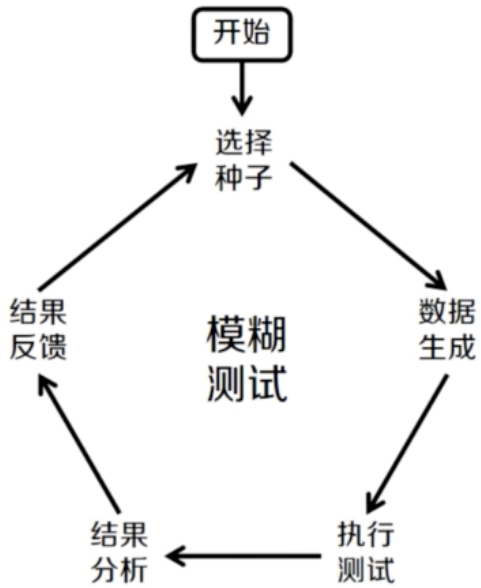
\includegraphics[width=0.97\linewidth]{images/模糊测试流程.png}
        \end{minipage}
    }
    \hspace{1em}
    \subfloat{
	    \begin{minipage}[t]{0.7\linewidth}
	    \centering
	    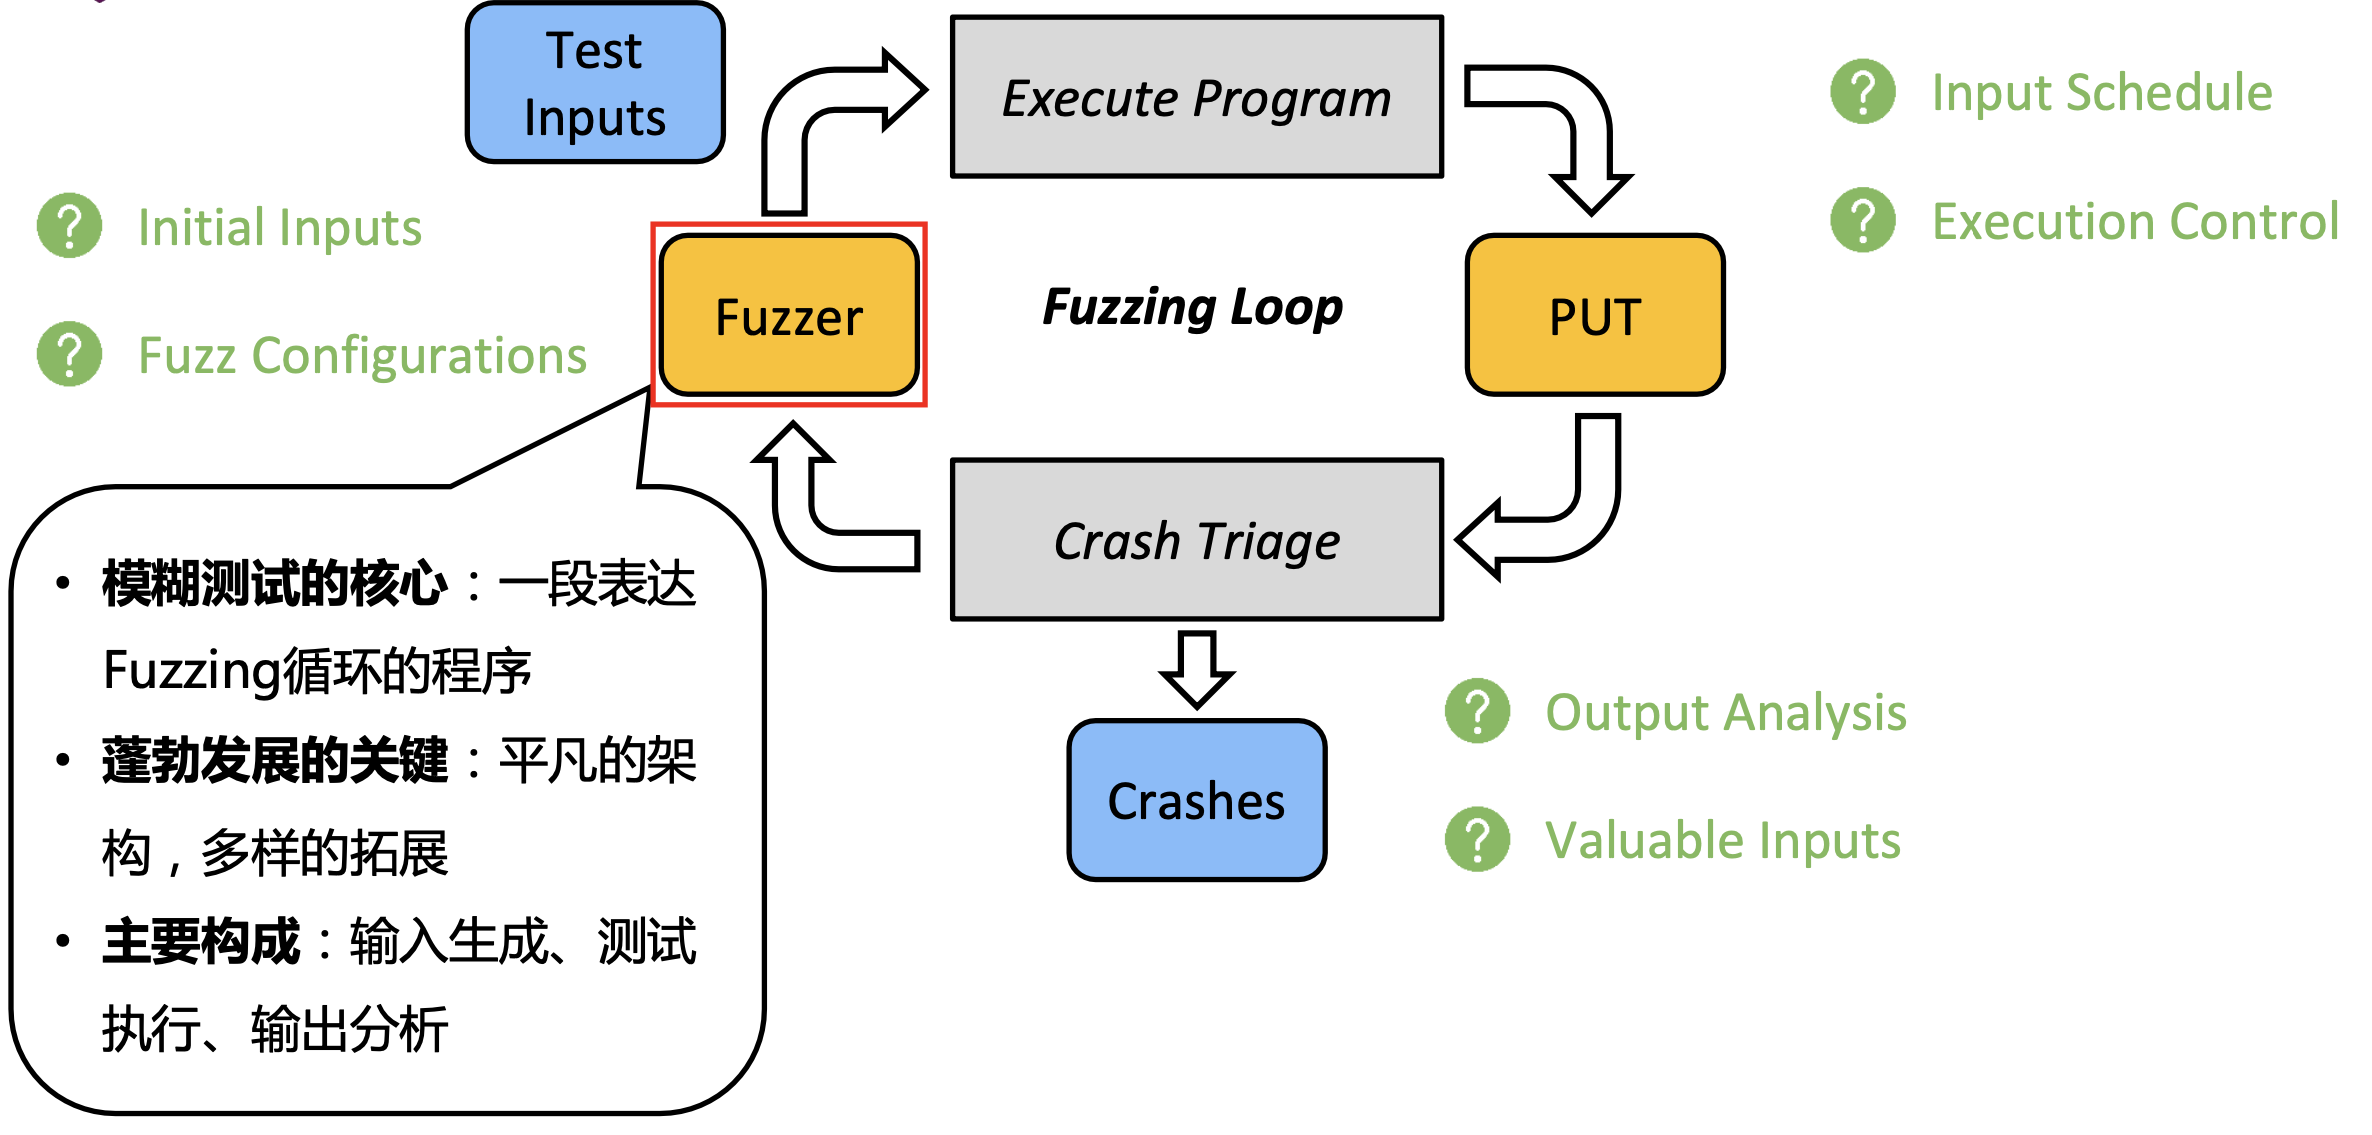
\includegraphics[width=0.97\linewidth]{images/模糊测试框架1.png}
	    \end{minipage}
	}
\end{figure}

\begin{figure}[H]
    \vspace{-0.5em}
	\centering
	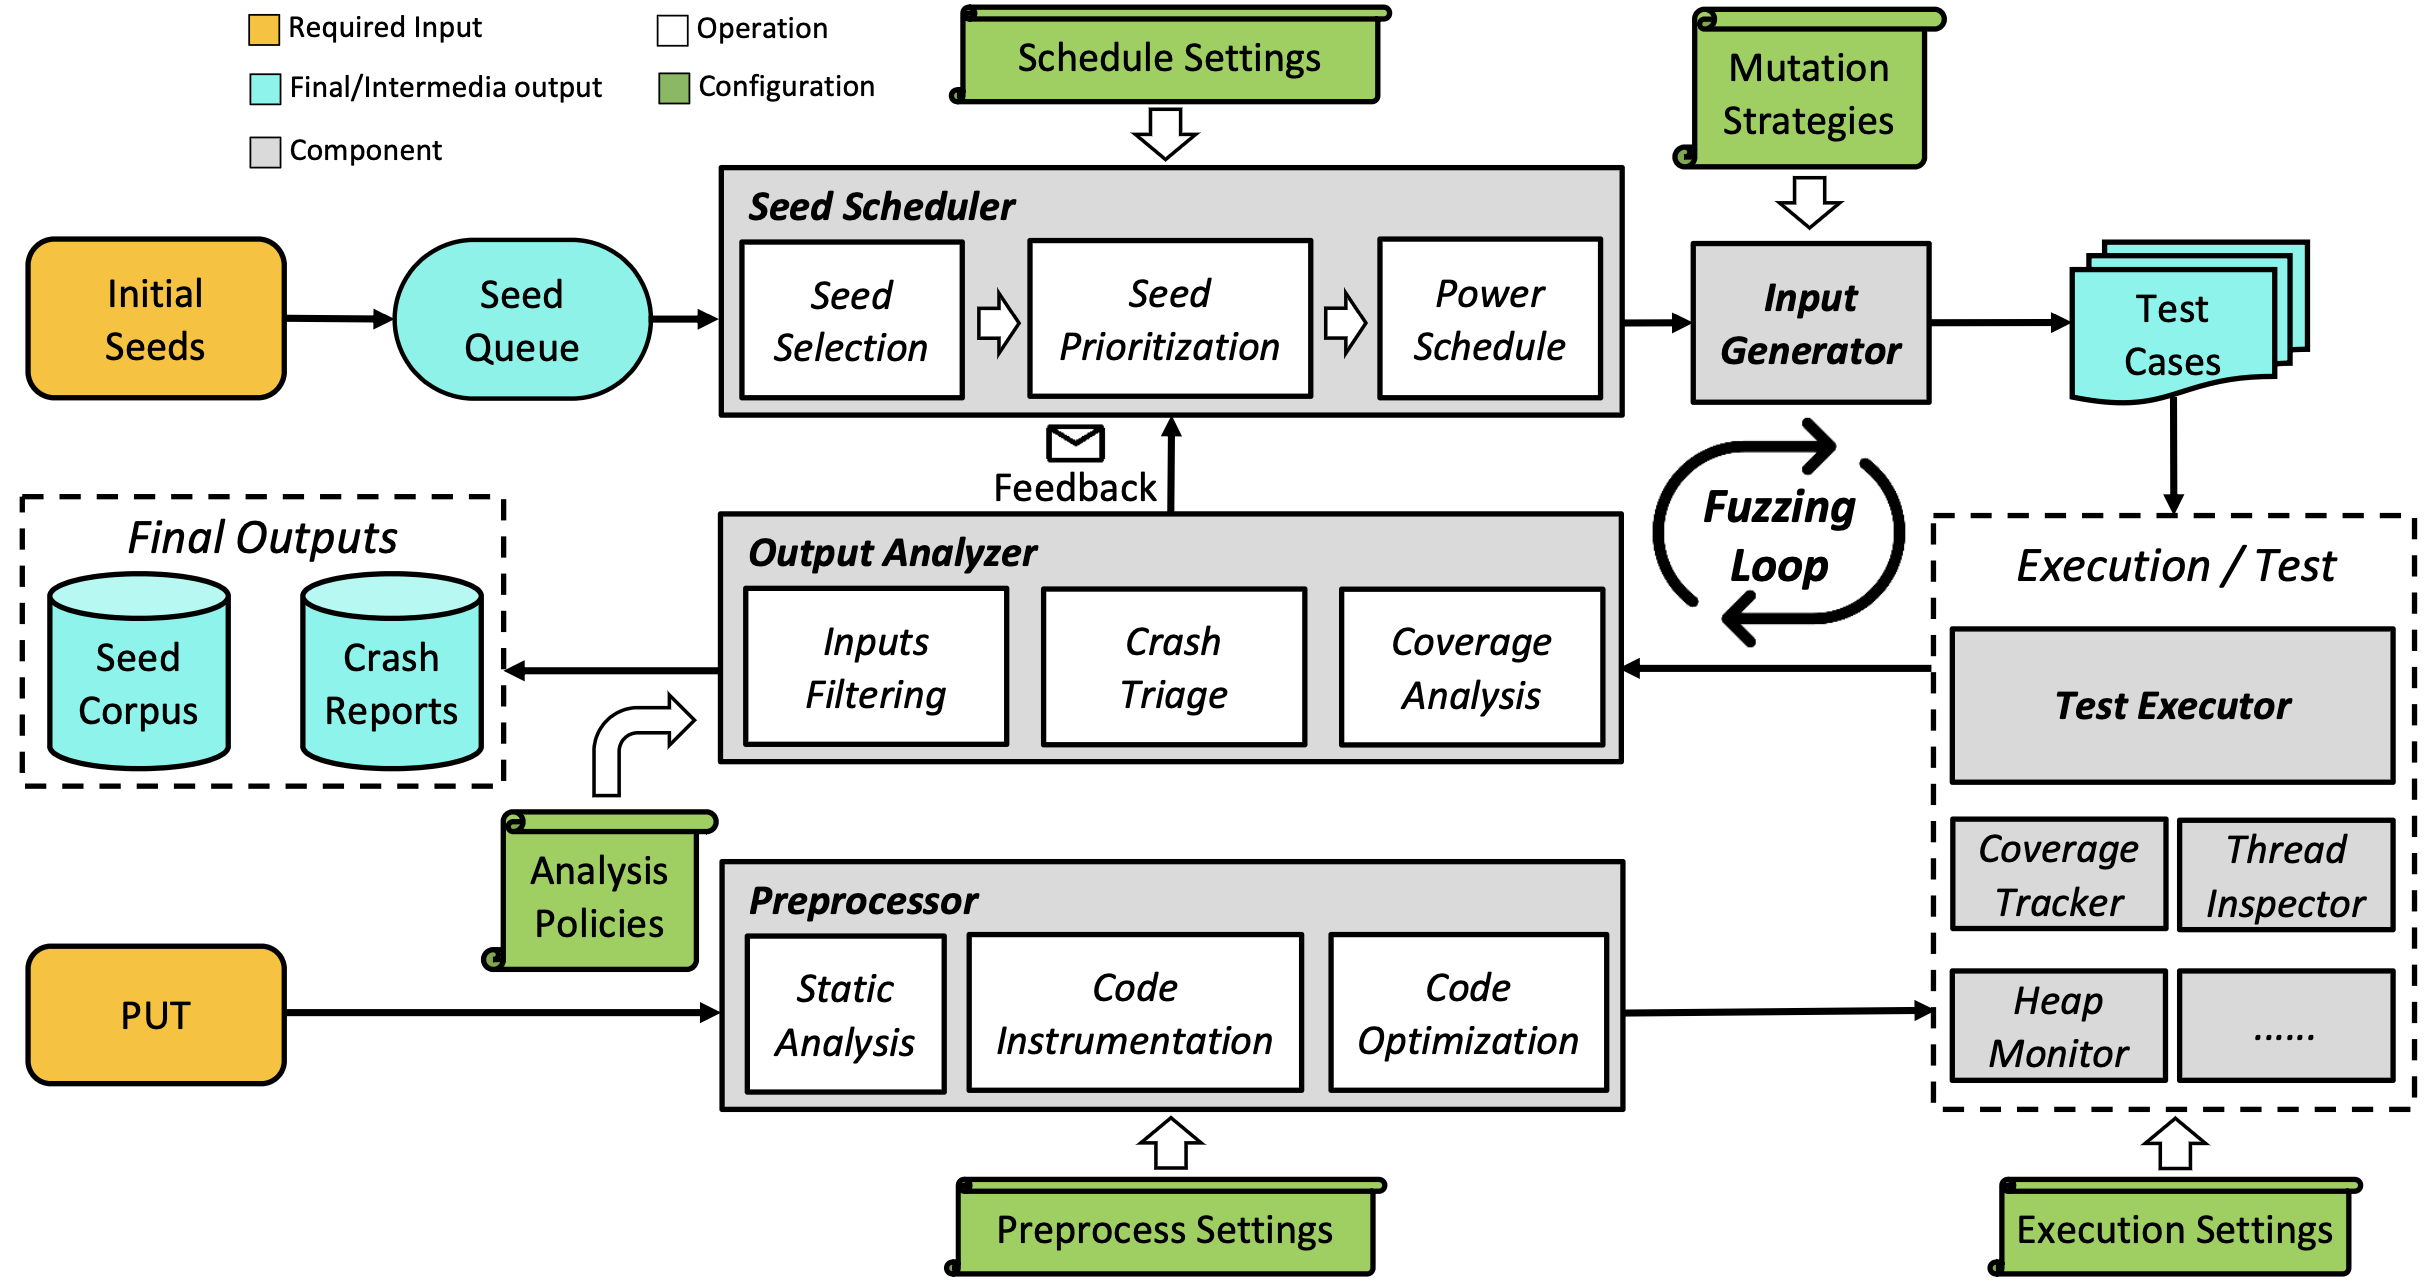
\includegraphics[width=0.85\textwidth]{images/模糊测试框架2.png}
    \vspace{-1em}
\end{figure}

模糊测试监测内容:程序中的哪些现象能够帮助判断是否存在问题
\vspace{-0.5em}
\begin{multicols}{2}
    \begin{itemize}
        \item 断言失败
        \item 异常崩溃
        \item 无效输入
        \item 错误输出
    \end{itemize}
\end{multicols}
\vspace{-1em}

\subsection{基于灰盒的模糊测试流程}
\begin{figure}[H]
    \vspace{-0.5em}
	\centering
	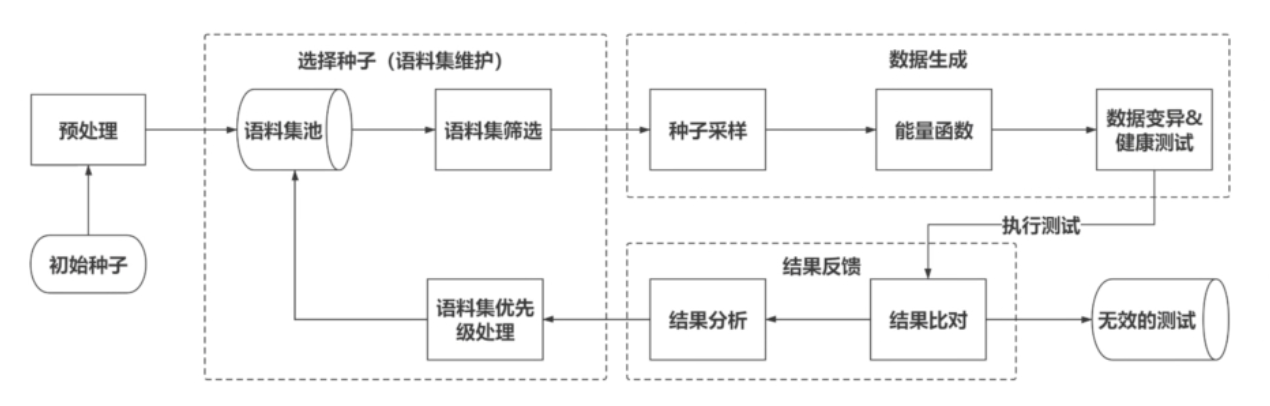
\includegraphics[width=0.95\textwidth]{images/基于灰盒的模糊测试流程.png}
    \vspace{-1em}
\end{figure}

\begin{itemize}
    \item 初始种子:已有的测试用例或者已知的符合所要测试程序输入范围的数据 
    \item 预处理:种子经过一定的预处理(比如编码转换或图像裁剪)使得种子满足程序的输入条件或参数要求
    \item 语料集:由于对测试用例数量和质量的要求,一般会将种子打包形成语料集
    \item 种子采样:根据模糊测试变异方法从送入过程引导的语料集中形成符合变异方法输入的种子元组
    \item 能量函数:旨在通过对语料集进行变异成功率检测实现在同样的测试计算资源尽可能生成多的能够成功变异的测试数据 
    \item 数据变异:根据所选用的变异方法,对选取的原始测试数据施加扰动,生成新的测试输入
    \item 与结果参照物(理论上应该得到的结果)对比或者是否发生崩溃
    \begin{itemize}
        \item 大多数情况用覆盖率分析来指导语料集的进一步优化
    \end{itemize}
\end{itemize}

AI模糊测试流程与传统模糊测试流程类似
\begin{itemize}
    \item 结果反馈和结果分析都由深度学习模型提供
    \item 模型同时指导语料集的维护
\end{itemize}

\subsection{算子差分模糊测试}
方法:将差分测试与模糊测试相结合
\begin{itemize}
    \item 引入值运算运用于算子接口,首先针对每个新生成测试用例,分别获取算子接口的中间过程值和返回值。
    \item 接着对输入参数、中间值和返回值进行处理。
    \item 然后对Tensor数据采用加权求和进行降维,井结合基本类型参数,最终得到一组覆盖值。
    \item 最后将新用例的一组覆盖值与语料集中所有已有元素的覆盖值进行比较,如果最近距离大于某个阈值,则将新用例加入语料集。
    \item 在差分测试的指导下,通过不同框架间的距离标准或精度标准来测量算子接口的结果。
\end{itemize}
